\documentclass[11pt]{article} 
\usepackage{geometry}
\geometry{letterpaper}

\usepackage{graphicx}   
\usepackage{amssymb}
\usepackage{tabularx}
\usepackage{float}
\usepackage{../latex/framed}
\usepackage{hyperref}
\hypersetup{
    colorlinks,
    citecolor=black,
    filecolor=black,
    linkcolor=black,
    urlcolor=blue
}

\usepackage[english]{babel}

\begin{document}

\begin{titlepage}
	\newcommand{\HRule}{\rule{\linewidth}{0.2mm}}
	\begin{center}
	\textsc{\LARGE McMaster University}\\[1.5cm]
	
	\textsc{\Large SmartServe}\\[0.5cm]
	\textsc{\large Software \& Mechatronics Capstone}\\[0.5cm] 

	\HRule\\[0.4cm]
		{\huge\bfseries Development Process \& Implementation}\\[0.4cm]
	\HRule\\[0.4cm]
	
	\begin{minipage}[t][][t]{0.5\textwidth}
		\begin{flushleft} \large
			\emph{Authors:}\\
			Christopher McDonald\\
			Harit Patel \\
			Janak Patel \\
			Jared Rayner  \\
			Nisarg Patel  \\
			Sam Hamel \\
			Sharon Platkin \\
		\end{flushleft}
	\end{minipage}
	~
	\begin{minipage}[t][][t]{0.4\textwidth}
		\begin{flushright} \large
			\emph{Professor:} \\
			Dr. Alan Wassyng \\[0.4cm]
			\emph{Teaching Assistants:} \\
			Bennett Mackenzie \\ 
			Nicholas Annable \\ 
			Stephen Wynn-Williams \\ 
			Viktor Smirnov
		\end{flushright}
	\end{minipage}\\[2cm]
	
	
\includegraphics[width=0.3\textwidth]{logo.png} \\
	{\large Last compiled on \today}
	\end{center}

\end{titlepage}

\tableofcontents
\listoffigures

\vfill
\begin{figure}[htbp]
   \centering
   \noindent\begin{tabularx}{\textwidth}{| >{\centering\arraybackslash}m{0.2\textwidth} | >{\centering\arraybackslash}m{0.2\textwidth} | >{\centering\arraybackslash}m{0.2\textwidth} | >{\centering\arraybackslash}m{0.285\textwidth} |}
   \hline 
   \textbf{Date} & \textbf{Revision} & \textbf{Comments} & \textbf{Author(s)} \\
   \hline
   October 28, 2017 & 1.0 & Added structure and content & Christopher McDonald \\ \hline
   October 30, 2017 & 1.1 & Added detail into Version Control section and revised document & Sharon Platkin \& Christopher McDonald \\ \hline
   \end{tabularx}
   \caption{Revision History}
\end{figure}

\newpage

\section{Introduction}
\subsection{Project Overview}
SmartServe is an autonomous table tennis training system for a wide range of table tennis players to aid in diagnosing and improving their performance. The system does so by shooting balls toward the player and detecting successful returns. It can then adapt to the player's weaknesses and expose them by playing more to them over time. This alleviates problems of finding and working with a coach or training many players in a short amount of time. The system will be deemed a success if table tennis players enjoy and can see value in using our system in place of or in tandem to a coach.\\\\
The development started at the beginning of the Fall 2017 academic turn and will conclude at the end of the Winter 2018 term. The team was assembled in the capstone course for Software and Mechatronics Engineering disciplines.
\subsection{Naming Conventions \& Terminology}
\begin{itemize}
\item \textbf{Git}: a distributed versioning control system
\item \textbf{Master Branch}: the main branch of the GitHub repository
\item \textbf{PR}: pull request, a request to add changes from one branch into another done via a merge commit or rebase
\item \textbf{Slack}: a messaging platform for teams to subscribe and publish to channels or send messages between two or more team members
\item \textbf{DevOps}: development operations
\end{itemize}

\section{Team Members}
The team members are as follows:
\begin{itemize}
\item Christopher McDonald
\item Harit Patel
\item Janak Patel
\item Jared Rayner
\item Nisarg Patel
\item Sam Hamel
\item Sharon Platkin
\end{itemize}
In addition to the list above, Dr. Alan Wassyng will be the Project Advisor. He will be assisted by Bennett Mackenzie, Nicholas Annable, Stephen Wynn-Williams and Viktor Smirnov for marking and providing advice to the team.
\subsection{Roles \& Responsibilities}
See Table \ref{rr} for a breakdown of roles and responsibilities. When a backup member is needed, they will be listed in italics.
\begin{table}[H] % TODO maybe fix table?
\centering
\caption{Roles \& Responsibilities Breakdown} 
\label{rr}
\begin{tabularx}{\textwidth}{| l | p{4cm} | X |}
\hline
Role & Member(s) & Responsibility \\ \hline
Scribe & Sharon Platkin \newline \textit{Jared Rayner} & Taking notes for all meetings \newline Posting notes to Slack after meetings \newline Booking rooms for team meetings  \\ \hline
DevOps Developer & Christopher McDonald \newline \textit{Sharon Platkin} & Solving issues related to GitHub \newline Configuring CI Tools \newline Merging code changes into the \textit{master} branch  \\ \hline
Team Contact & Christopher McDonald \newline \textit{Nisarg Patel} & Handle a majority of communication with Project Advisor and Teaching Assistants \\ \hline
Hardware Team Member & Janak Patel \newline Jared Rayner \newline Nisarg Patel & Handle most hardware focused work tasks \\ \hline
Software Team Member & Christopher McDonald \newline Harit Patel \newline Sam Hamel \newline Sharon Platkin & Handle most software focused work tasks \\ \hline
\end{tabularx}
\end{table}
\subsection{Meeting Schedule}
The team currently has weekly meetings scheduled on Tuesdays at 16:30 and Fridays at 16:30 for a duration of 50 minutes. Every member of the team is expected to attend. Every other Tuesday meeting must cover reflecting on the previous 2 weeks and planning the following 2 weeks for what work needs to be done in that time. All other meetings will be for progress updates, clarifying any work going forward and removing roadblocks which inhibit optimal performance. \\ \\
The Hardware and Software team will schedule meetings on an ad hoc basis, inviting any members which have a stake in the content being discussed. In the event Sharon Platkin is not present and therefore cannot be the Scribe, a member will be elected by and among the attendees.
\subsection{Communication Pipelines}
All inter-team communication will be done through Slack. This will allow team members to communicate via channels or groups. Examples of the channels currently used are \textit{hardware}, \textit{software}, \textit{documentation}, \textit{meetings}, \textit{deliverables} and \textit{git}. The \textit{git} channel will give updates on every open PR (Pull Request) and the \textit{deliverables} channel gives reminders 2 days prior to deliverable deadlines. Meeting notes will be posted in the \textit{meetings} channel. \\ \\
When communicating with the TAs or Project Advisor, email will be used and the Team Contact will relay all relevant information to all other team members.
\subsection{Handling Change}
In the event any aspect of the project must be changed, all members can be involved in the decision making. In the absence of a unanimous decision, the team must decide if the change is paramount to the outcome of the project. If not, the decision will be left to a vote by all meeting attendees. If so, a teaching assistant will be involved in the decision making to aid in arriving to a unanimous decision. The Project Advisor will also be involved at the discretion of the teaching assistant. \\ \\
Once the change has been decided, all documentation and code changes will be given the highest priority to reflect the change made. This will ensure no further work will be done using documentation or code that does not reflect the team's ideals.
\section{Version Control}
\subsection{Technology}
The technology used for version control will be \textit{git}. The \textit{git} repository will be hosted by GitHub and can be found \href{https://github.com/ChristopherMcDonald/SoftwareTronCapstone}{here}. \textit{Git} allows developers to host a decentralized version of the source code for any project. This is in addition to a copy hosted on a remote repository. This technology allows any number of developers to perform work on their own copy of the source without impeding on the other developers. Once a developer makes a complete set of changes, they can include these changes in a commit and push them to the remote repository.
\subsection{Workflow}
The workflow we will be using is a feature-branch workflow with the addition of a two-stage release process. For all releases, changes will be made via a PR into the \textit{master} branch from the \textit{develop} branch. Therefore, any demonstrations and deliverables can be found by checking out the \textit{master} branch. When making any changes, an ad hoc branch will be made off the \textit{dev} branch. Once completed, a PR can be made from that branch into the \textit{develop} branch. This pertains to documentation and source code. A flowchart for this can be found in Figure \ref{fig:git}. Once a developer begins working on any item, they will start by making a branch based off of \textit{develop}. \\\\
In the event commits have been added to \textit{develop} after making your branch and before merging it into develop, a rebase will be required. This will effectively place all your commits made to your feature branch, onto the current \textit{develop} branch.
\begin{figure}[htbp]
   \centering
   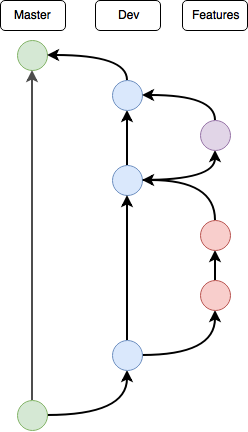
\includegraphics[width=0.7\textwidth]{img/git.png} % requires the graphicx package
   \caption{Feature-Branch and Develop Git Workflow}
   \label{fig:git}
\end{figure}
\subsection{Setup}
The following steps must be taken to contribute to the source code.
\begin{itemize}

\item Clone the Project
\begin{verbatim}
git clone https://github.com/ChristopherMcDonald/SoftwareTronCapstone.git
\end{verbatim}

\item Add a Feature Branch
\begin{verbatim}
cd /path/to/repo
git fetch --all
git checkout develop
git checkout -b BRANCH_NAME
\end{verbatim}

\item Push Changes to Repository
\begin{verbatim}
git add FILE_NAME
git commit -m "MESSAGE"
git push # for first push, git push --set-upstream origin BRANCH_NAME
\end{verbatim}

\item Rebase Against \textit{develop} Branch
\begin{verbatim}
git fetch --all
git rebase develop
# deal with any conflicts
git push -f
\end{verbatim}

\end{itemize}

\subsection{Versioning Scheme}
When items of this system are added or revised, the version number of the system will be updated. This number will follow the\textit{major.minor.patch} versioning scheme. This means when anything major has changed, such as a feature being added or a specification being changed, it will increment the current \textit{major} number by one. \textit{Minor} updates will include changes of items in order to refine a feature or meet a specification and will also be incremented by one. For any bug fixes or commentary changes, the \textit{patch} number will be incremented by one.


\section{Process Workflow}
In order to facilitate the development of the system, work will be organized into 2-week long sessions. At the beginning of the week, the team will consider the next 2-3 deliverables and schedule them in accordingly. The team will attempt to finish each deliverable a week or more before the deadline. This allows the team to be ahead of schedule and gives them the ability to respond to other items should they arise. During meetings before the end of each 2-week session, any priorities will be adjusted as needed. When the work session is completed, items will be placed into the next session or placed in the backlog until further consideration. \\\\
For the hardware design and assembly of the system, the team is currently using a rapid prototyping approach similar to the cycle in Figure \ref{fig:rapid}. This allows the team to quickly develop and build prototypes for parts of the system. Instead of building everything at once, portions of the system will be built incrementally and integrated into each other to form our complete system. We are also utilizing the agile methodology in conjunction with rapid prototyping to allow sections of the system to be designed and built simultaneously. This approach is beneficial because it gives more opportunities to obtain feedback from TAs or Dr. Alan Wassyng to further refine the prototype. The team is using ready made parts and 3D printing for prototype development because it allows for quick changes and improvements to the prototype which will eventually be implement into the final system.
\begin{figure}
	\centering
	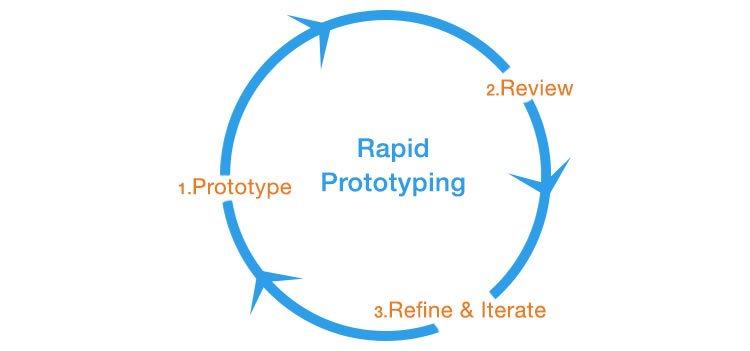
\includegraphics[width=0.7\textwidth]{effective-rapid-prototyping-diagram}
	\caption{Rapid Prototyping Development Processes}
	\label{fig:rapid}
\end{figure}
\section{Onboarding Process}
The following administrative work must be done to onboard another team member:
\begin{itemize}
\item Invite them to Slack team
\item Share team's Google Calendar with them
\item Add them as a collaborator on GitHub
\item Add them to the list of authors on the documentation template
\end{itemize}
The new member will be expected to read all current revisions of documentation made for the project. Any questions which arise can be asked during meetings or on Slack. After a comprehensive understanding of the project, tasks can be assigned to them and any education will be done on an ad hoc basis. \\\\
The following tools will need to be installed by the member with the help of the DevOps developer:
\begin{itemize}
\item Git version 2.14.0 found \href{https://git-scm.com}{here}
\item LaTeX version \LaTeX  $2_\varepsilon$ found \href{https://www.latex-project.org/get/}{here}
\end{itemize}
\end{document}  